\documentclass[oneside,14pt]{book}

\usepackage[T1,T2A]{fontenc}
\usepackage[utf8]{inputenc}
\usepackage[english,russian]{babel}
\usepackage{indentfirst}

%\usepackage[paperwidth=15cm,paperheight=7.5cm]{geometry} % планшет
%\usepackage[paperwidth=297mm,paperheight=210mm]{geometry} % A4
%\usepackage[paperwidth=148mm,paperheight=105mm]{geometry} % A5
\usepackage[paperwidth=18cm,paperheight=13cm,margin=5mm]{geometry} % экран*2

%\usepackage[colorlinks=true,
%]{hyperref}
%\newcommand{\email}[2]{#1\ \href{mailto:#2}{<\nolinkurl{#2}>}}
% %\newcommand{\email}[2]{\emph{#1\ <#2>}}
\usepackage[unicode,colorlinks,
pdftitle={Azbuka ARMaturschika (ru)},
pdfauthor={(c) Dmitry Ponyatov <dponyatov@gmail.com>, SSAU ASCL},
pdfsubject={ru manual on writing programs for Cortex-M MCUs},
pdfkeywords={ARM} {Cortex} {MCU} {ARMatura} {Arduino} {SSAU}
]{hyperref}

\usepackage{wrapfig}
\usepackage{graphicx}
\usepackage{epstopdf}
\DeclareGraphicsExtensions{.eps}

\usepackage{listings}
\usepackage{dirtree}
\usepackage[usenames,dvipsnames,svgnames]{xcolor}
\newcommand{\cppcolor}{\color[rgb]{0.94, 0.97, 1.0}} % Alice blue
\newcommand{\asmcolor}{\color[rgb]{0.98, 0.92, 0.84}} % Antique white
\newcommand{\ldcolor}{\color[rgb]{0.67, 0.9, 0.93}} % Blizzard Blue
\newcommand{\concolor}{\color[rgb]{0.88, 1.0, 1.0}} % Light cyan
\newcommand{\makecolor}{\color[rgb]{0.9, 0.9, 0.98}} % Lavender mist

%\definecolor{cppcolor}{rgb}{0.94, 0.97, 1.0}
\lstset{frame=single,
numbers=left, numberstyle=\small, numbersep=1mm,
tabsize=4,
keywordstyle=\color{blue}\texttt,
commentstyle=\color{cyan}\texttt,
inputencoding=utf8, extendedchars=true, showspaces=false,  
inputencoding=cp1251
}
\usepackage{lstlangarm}
\usepackage{lstlanggnumake}
\usepackage{lstlanggnuld}
\usepackage{lstlanggnudump}

\lstdefinestyle{cpp}{language=C++,backgroundcolor=\cppcolor}
\lstdefinestyle{asm}{language={[ARM]Assembler},backgroundcolor=\asmcolor}
\lstdefinestyle{gnuld}{language={[GNU]Link},backgroundcolor=\ldcolor}
\lstdefinestyle{con}{backgroundcolor=\concolor}
\lstdefinestyle{mk}{language=[GNU]Make,backgroundcolor=\makecolor}
\lstdefinestyle{objdump}{language=[GNU]Dump}

\newcommand{\cm}[1]{Cortex-M#1}
\newcommand{\cx}{\cm{x}}

\newcommand{\vld}{STM32VLDISCOVERY}

%\renewcommand{\url}[1]{\textbf{#1}}
\newcommand{\email}[1]{$<$\href{mailto:#1}{\textbf{#1}}$>$}

\newcommand{\cpp}{$C^{+^{+}}$}

\newcommand{\cp}[1]{\footnote{копипаста: #1}}

\newcommand{\thmod}{Thumb}
\newcommand{\armod}{ARM}
\newcommand{\arm}{ARM}

\newcommand{\Reg}[1]{\textbf{#1}}
\newcommand{\R}[1]{\Reg{R#1}}

\newcommand{\periph}[1]{\texttt{#1}}
\newcommand{\jtag}{\periph{JTAG}}

\usepackage{wasysym} % smileys
\usepackage{gensymb} % celsius
\usepackage{amssymb} % windows key
\usepackage{textcomp} % bigcircle

\usepackage[os=win]{menukeys}
\newcommand{\winstart}{$\boxplus$}
\newcommand{\file}[1]{\textbf{\textsf{#1}}}
\newcommand{\window}[1]{\textbf{\textit{#1}}}
\newcommand{\alarm}[1]{{\color{DarkRed}#1}}
\newcommand{\wcmd}[1]{\keys{\winstart+R}\ \directory{#1}}
\newcommand{\checkbox}{$\boxtimes$}
\newcommand{\uncheckbox}{$\square$}
\newcommand{\lms}{\keys{$\lhd$}}
\newcommand{\rms}{\keys{$\rhd$}}
\newcommand{\eclpx}{\window{Project Explorer}}

\newcommand{\win}[1]{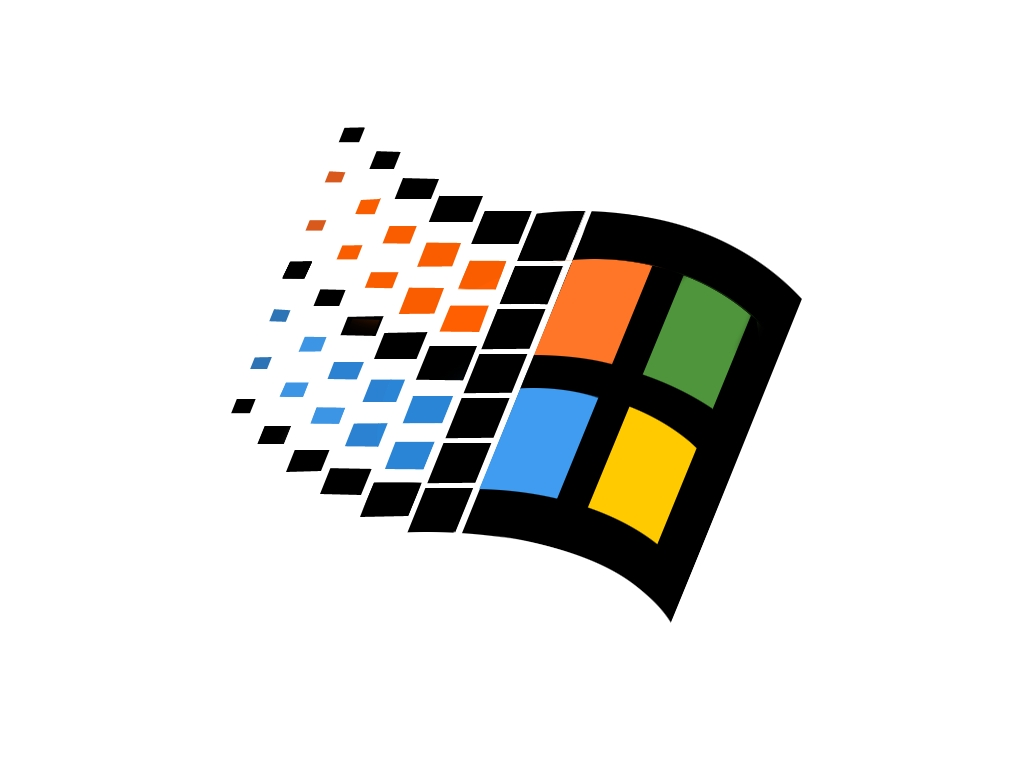
\includegraphics[height=10ex]{fig/winlogo.jpg} #1}
\newcommand{\lin}[1]{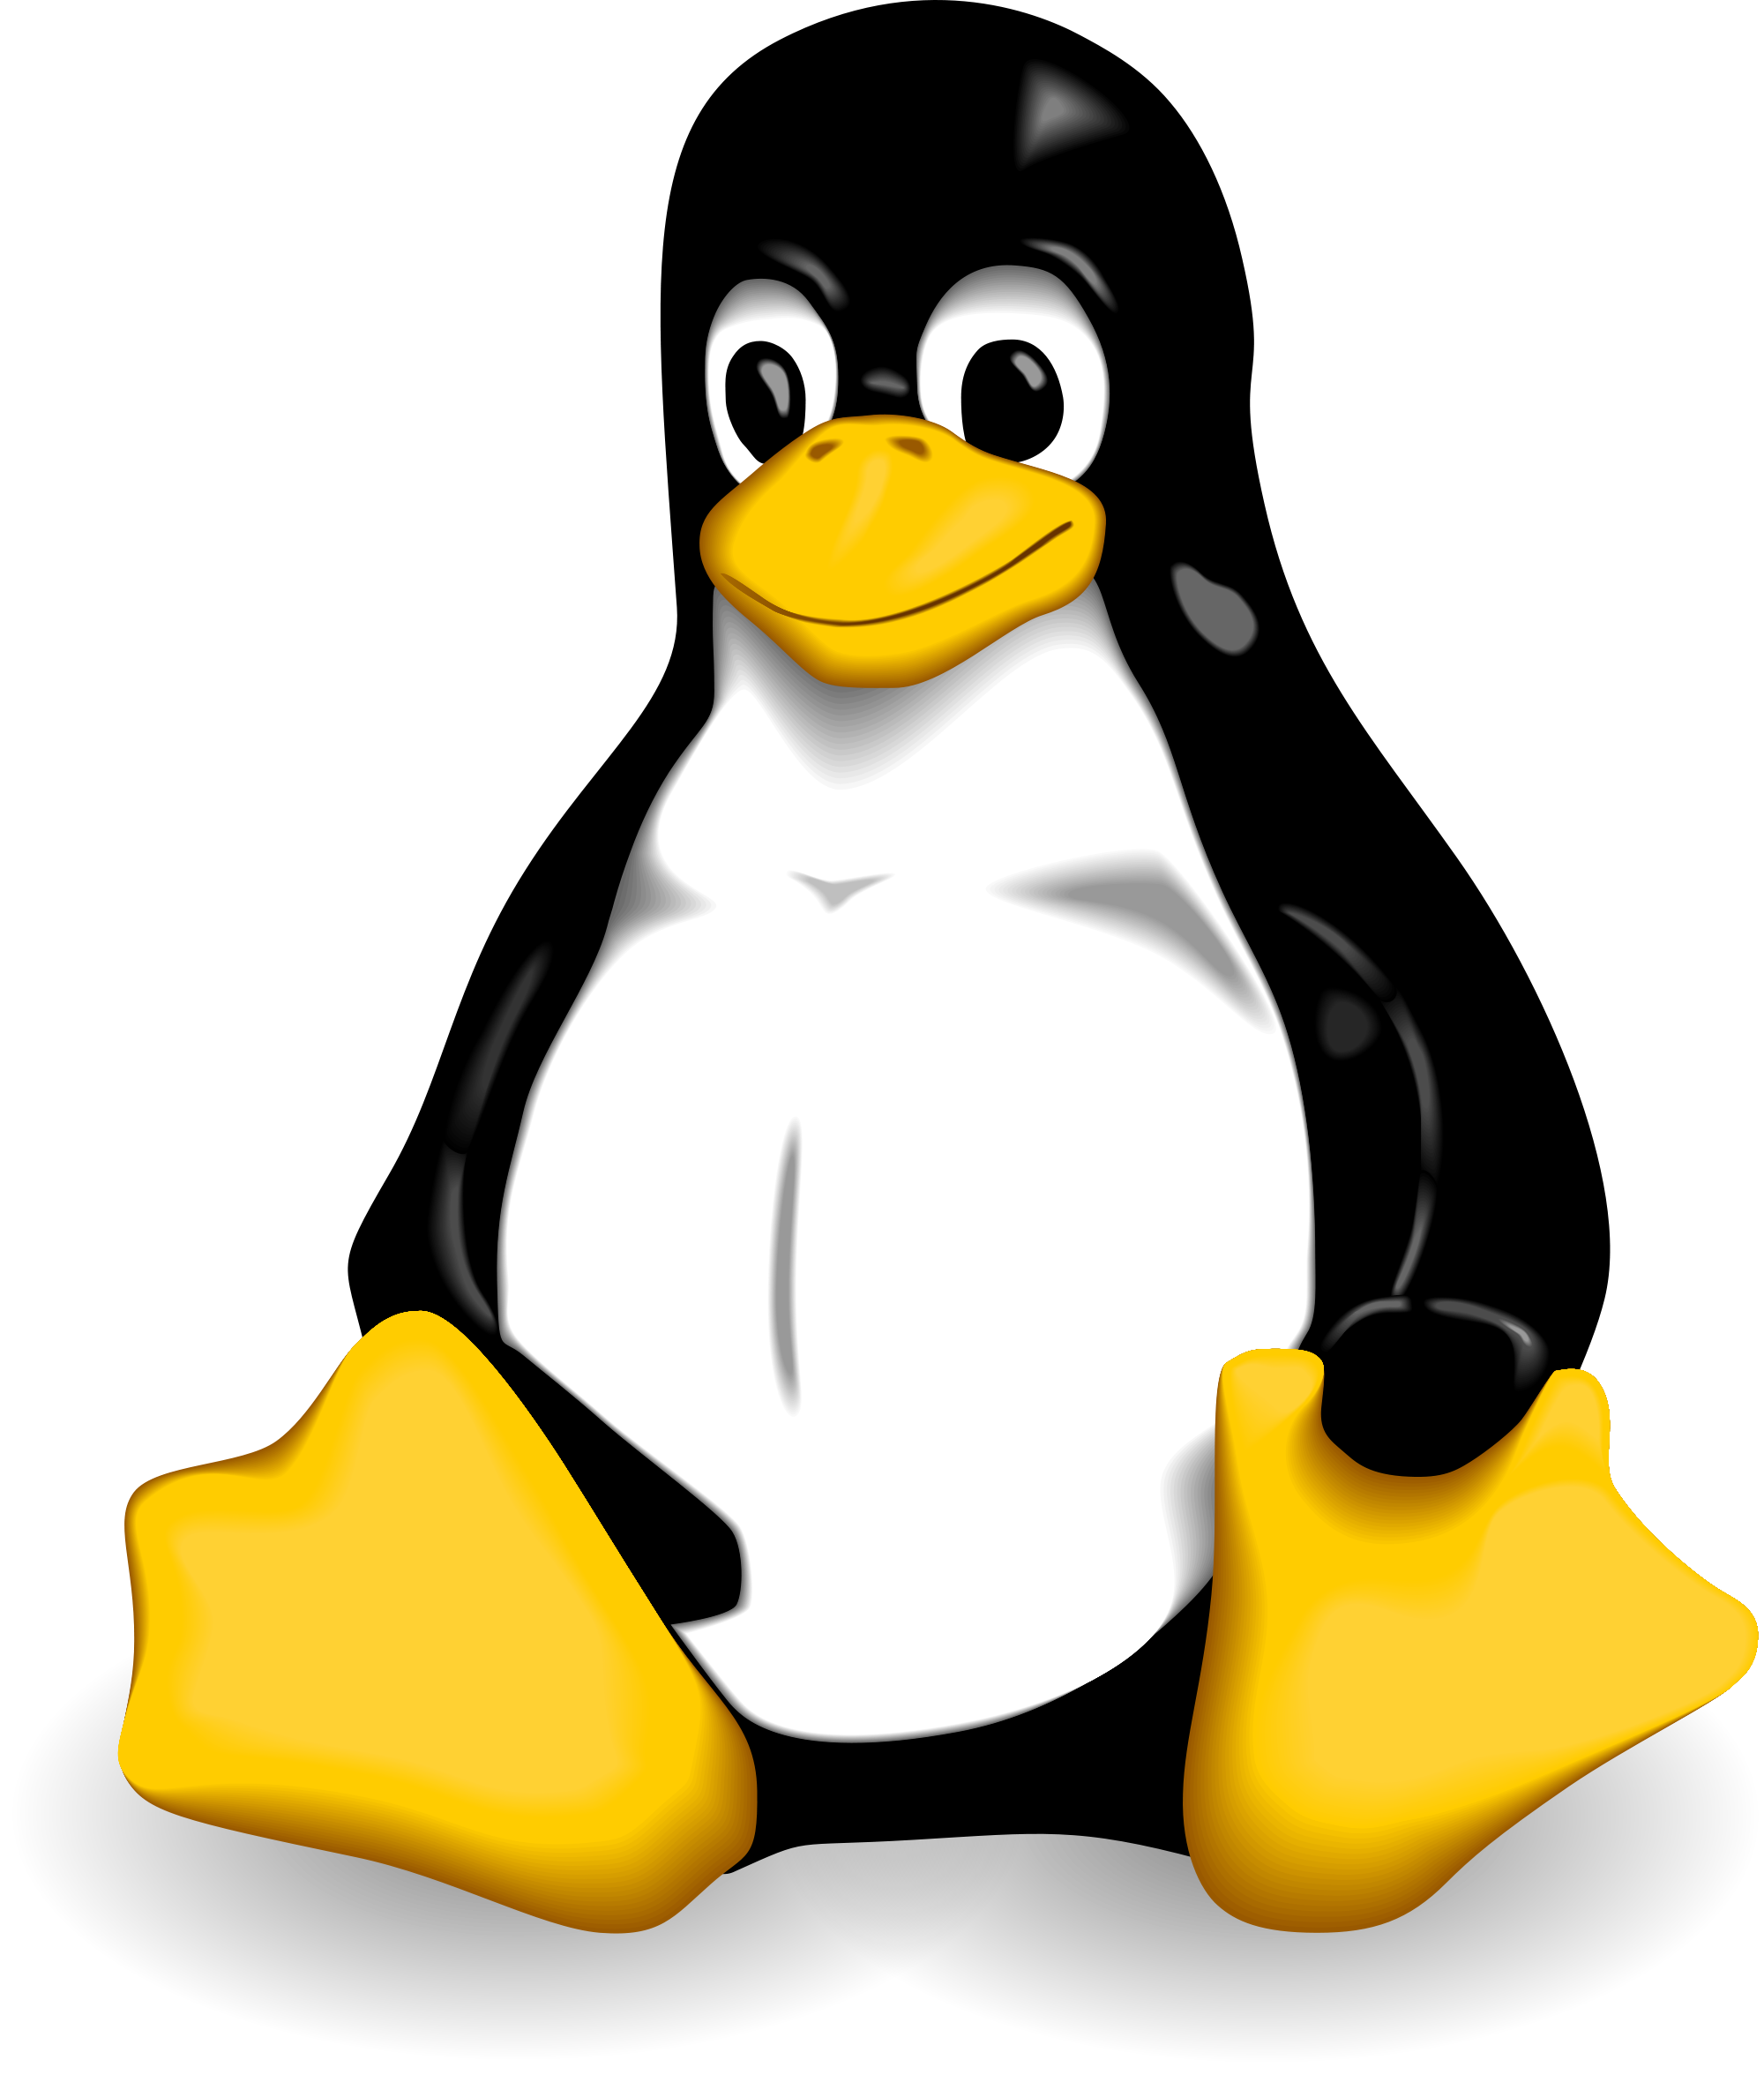
\includegraphics[height=10ex]{fig/linuxcolor.png} #1}
\newcommand{\bug}{
\includegraphics[height=10ex]{fig/iconbug.png}}

\newcommand{\linux}{Linux}
\newcommand{\git}{Git}
\newcommand{\eclipse}{\textcircled{$\equiv$}\textsc{eclipse}}
%\newcommand{\term}[1]{\underline{#1}}
\newcommand{\term}[1]{\underline{\color{DarkBlue} #1}}
\newcommand{\miktex}{MiK\TeX}
\newcommand{\internet}{Internet}
\newcommand{\ql}{Quantum$^{\circledR}L^{e}aPs$}
\newcommand{\gdb}{GDB}

\newcommand{\make}{\file{make}}
\newcommand{\makefile}{\file{Makefile}}

\usepackage{tocloft}
\newcommand{\listlabname}{Лабораторные работы}
\newlistof{lab}{ex}{\listlabname}
\newcommand{\labpart}[1]{\addcontentsline{ex}{part}{#1}}
\newcounter{labworkcounter}
\newcommand{\labwork}[1]{
\refstepcounter{labworkcounter}
\section*{ЛР\thelabworkcounter: #1}
\addcontentsline{toc}{subsection}{ЛР\thelabworkcounter: #1}
\addcontentsline{ex}{section}{ЛР\thelabworkcounter: #1}
}
\newcommand{\labref}[1]{ЛР\ref{#1}}

\newcommand{\thetitle}{Азбука халтурщика-ARMатурщика}

\newcommand{\mytitle}[1]{
\title{\Huge{\thetitle}\\
#1\\
\normalsize{учебный курс по микроконтроллерам \cx:\\
Миландр 1986ВЕ, STM32F, LPC21xx}}
}

\author{(copypasta) Понятов Д.А. \email{dponyatov@gmail.com}, ИКП СГАУ}


\begin{document}

\mytitle{\ }
\maketitle
\tableofcontents
\listoflab

\part{Обзор семейства микроконтроллеров \cx}

\chapter{Архитектура ARM}

\cp{\url{http://ru.wikipedia.org/wiki/ARM}} %\_(архитектура)

Архитектура ARM (Advanced RISC Machine, Acorn RISC Machine, 
усовершенствованная RISC-машина)\ --- семейство лицензируемых 32-битных и 
64-битных микропроцессорных ядер разработки компании ARM Limited.

Среди лицензиатов: практически все заметные разработчики цифровых
электронных компонентов.
Многие лицензиаты делают собственные версии ядер на базе ARM.

Значимые семейства процессоров: ARM7, ARM9, ARM11 и Cortex.

В 2007 году около 98\% из более чем миллиарда мобильных телефонов, продаваемых 
ежегодно, были оснащены по крайней мере одним процессором ARM. По состоянию 
на 2009 на процессоры ARM приходилось до 90\% всех встроенных 32-разрядных 
процессоров. Процессоры ARM широко используются в потребительской 
электронике\ --- в том числе КПК, мобильных телефонах, цифровых носителях и 
плеерах, портативных игровых консолях, калькуляторах и компьютерных п
ериферийных устройствах, таких как жесткие диски или маршрутизаторы.

Эти процессоры имеют низкое энергопотребление, поэтому находят широкое 
применение во встраиваемых системах и преобладают на рынке мобильных 
устройств, для которых данный фактор немаловажен.

В настоящее время значимыми являются несколько семейств процессоров ARM:

\begin{itemize}
\item ARM7 (с тактовой частотой до 60-72 МГц), предназначенные, например, для 
недорогих мобильных телефонов и встраиваемых решений средней производительности. 
В настоящее время активно вытесняется новым семейством Cortex.
\item ARM9, ARM11 (с частотами до 1 ГГц) для продвинутых телефонов, карманных 
компьютеров и встраиваемых решений высокой производительности.
\item Cortex A\ --- новое семейство процессоров на смену ARM9 и ARM11.
\item Cortex M\ --- новое семейство процессоров на смену ARM7, также 
призванное занять новую для ARM нишу встраиваемых решений низкой 
производительности. В семействе присутствуют три значимых ядра: \cm{0}, 
\cm{3} и \cm{4}.
\end{itemize}

\paragraph{Архитектура}

Существует спецификация архитектуры ARM Cortex, которая разграничивает все типы опций, 
которые поддерживает ARM, так как детали реализации каждого типа процессора м
огут отличаться. Архитектура развивалась с течением времени, и начиная с 
ARMv7 были определены 3 профиля:
\begin{itemize}
\item{A (application)} для устройств, требующих высокой производительности (смартфоны, планшеты)
\item{R (real time)} для приложений, работающих в реальном времени,
\item{M (microcontroller)} для микроконтроллеров и недорогих встраиваемых устройств.
\end{itemize}

\paragraph{Режимы процессора}

Процессор может находиться в одном из следующих рабочих режимов:
\begin{itemize}
\item{User mode} — обычный режим выполнения программ. В этом режиме 
выполняется большинство программ.
\item{Fast Interrupt (FIQ)} — режим быстрого прерывания (меньшее время с
рабатывания)
\item{Interrupt (IRQ)} — основной режим прерывания.
\item{System mode} — защищённый режим для использования операционной системой.
\item{Abort mode} — режим, в который процессор переходит при возникновении 
ошибки доступа к памяти (доступ к данным или к инструкции на этапе 
prefetch конвейера).
\item{Supervisor mode} — привилегированный пользовательский режим.
\item{Undefined mode} — режим, в который процессор входит при попытке 
выполнить неизвестную ему инструкцию.
\end{itemize}

Переключение режима процессора происходит при возникновении соответствующего 
исключения, или же модификацией регистра статуса.

\paragraph{Набор команд ARM}

Режим, в котором исполняется 32-битный набор команд.

\paragraph{Набор команд \thmod}

Для улучшения плотности кода процессоры, начиная с ARM7TDMI, снабжены режимом 
\thmod. В этом режиме процессор выполняет альтернативный набор 16-битных 
команд. Большинство из этих 16-разрядных команд переводятся в нормальные 
команды ARM. Уменьшение длины команды достигается за счет сокрытия некоторых 
операндов и ограничения возможностей адресации по сравнению с режимом полного 
набора команд ARM.

В режиме \thmod\ меньшие коды операций обладают меньшей функциональностью. 
Например, только ветвления могут быть условными, и многие коды операций имеют 
ограничение на доступ только к половине главных регистров процессора. Более 
короткие коды операций в целом дают большую плотность кода, хотя некоторые 
операции требуют дополнительных команд. В ситуациях, когда порт памяти или 
ширина шины ограничены 16 битами, более короткие коды операций режима 
\thmod\ становятся гораздо производительнее по сравнению с обычным 32-битным ARM 
кодом, так как меньший программный код придется загружать в процессор при 
ограниченной пропускной способности памяти.

Аппаратные средства типа Game Boy Advance, как правило, имеют небольшой объём 
оперативной памяти доступной с полным 32-битным информационным каналом. Но 
большинство операций выполняется через 16-битный или более узкий информационный 
канал. В этом случае имеет смысл использовать \thmod\ код и вручную 
оптимизировать некоторые тяжелые участки кода, используя переключение в 
режим \armod.

\paragraph{Набор команд \thmod2}

\thmod2 — технология, стартовавшая с ARM1156 core, анонсированного в 2003 
году. Он расширяет ограниченный 16-битный набор команд Thumb дополнительными 
32-битными командами, чтобы задать набору команд дополнительную ширину. Цель 
\thmod2\ --- достичь плотности кода как у Thumb, и производительности как у 
набора команд \armod\ на 32 битах. Можно сказать, что в ARMv7 эта цель была 
достигнута.

\thmod2 расширяет как команды \armod, так и команды \thmod\ ещё большим 
количеством команд, включая управление битовым полем, табличное ветвление, 
условное исполнение. Новый язык «Unified Assembly Language» (UAL) поддерживает 
создание команд как для ARM, так и для Thumb из одного и того же исходного 
кода. Версии \thmod\ на ARMv7 выглядят как код ARM. Это требует осторожности и 
использования новой команды if-then, которая поддерживает исполнение до 4 
последовательных команд испытываемого состояния. Во время компиляции в ARM 
код она игнорируется, но во время компиляции в код \thmod2 генерирует команды.

\paragraph{Набор команд Jazelle}

Jazelle — это технология, которая позволяет байткоду Java исполняться прямо 
в архитектуре ARM в качестве 3-го состояния исполнения (и набора команд) 
наряду с обычными командами ARM и режимом Thumb. Поддержка технологии Jazelle 
обозначается буквой «J» в названии процессора — например, ARMv5TEJ. Данная 
технология поддерживается начиная с архитектуры ARMv6, хотя новые ядра 
содержат лишь ограниченные реализации, которые не поддерживают аппаратного 
ускорения.

\paragraph{ARMv8 и набор команд ARM 64 бит}

В конце 2011 года была опубликована новая версия архитектуры, ARMv8. В ней 
появилось определение архитектуры AArch64, в которой исполняется 64-битный 
набор команд A64. Поддержка 32-битных команд получила название A32 и
 исполняется на архитектурах AArch32. Инструкции Thumb поддерживаются в 
 режиме T32, только при использовании 32-битных архитектур. Допускается 
 исполнение 32-битных приложений в 64-битной ОС, и запуск виртуализованной 
 32-битной ОС при помощи 64-битного гипервизора.[47] Applied Micro, AMD, 
 Broadcom, Calxeda, HiSilicon, Samsung, STM и другие заявили о планах по 
 использованию ARMv8. Ядра Cortex-A53 и Cortex-A57, поддерживающие ARMv8, 
 были представлены компанией ARM 30 октября 2012 года.[48]

Как AArch32, так и AArch64, поддерживают VFPv3, VFPv4 и advanced SIMD (NEON). 
Также добавлены криптографические инструкции для работы с AES, SHA-1 и SHA-256.

\paragraph{Условное исполнение}

Одним из существенных отличий архитектуры ARM от других архитектур ЦПУ 
является так называемая предикация — возможность условного исполнения команд. 
Под «условным исполнением» здесь понимается то, что команда будет выполнена 
или проигнорирована в зависимости от текущего состояния флагов состояния 
процессора.

В то время как для других архитектур таким свойством, как правило, обладают 
только команды условных переходов, в архитектуру ARM была заложена 
возможность условного исполнения практически любой команды. Это было 
достигнуто добавлением в коды их инструкций особого 4-битового поля 
(предиката). Одно из его значений зарезервировано на то, что инструкция 
должна быть выполнена безусловно, а остальные кодируют то или иное сочетание 
условий (флагов). С одной стороны, с учётом ограниченности общей длины 
инструкции, это сократило число бит, доступных для кодирования смещения в 
командах обращения к памяти, но с другой — позволило избавляться от 
инструкций ветвления при генерации кода для небольших if-блоков.

Пример, обычно рассматриваемый для иллюстрации — основанный на вычитании 
алгоритм Евклида. В языке C он выглядит так:

\begin{lstlisting}[style=cpp,title={алгоритм Евклида}]
while (i != j) {
       if (i > j)
           i -= j;
       else
           j -= i;
}
\end{lstlisting}

А на ассемблере ARM — так:

\begin{lstlisting}[style=asm]
loop CMP Ri, Rj; set condition "NE" if (i != j),
						; "GT" if (i > j),
						; or "LT" if (i < j)
	SUBGT  Ri, Ri, Rj   ; if "GT" (greater than), i = i-j;
	SUBLT  Rj, Rj, Ri   ; if "LT" (less than), j = j-i;
	BNE    loop         ; if "NE" (not equal), then loop
\end{lstlisting}

Из кода видно, что использование предикации позволило полностью избежать 
ветвления в операторах else и then. Заметим, что если Ri и Rj равны, то ни 
одна из SUB инструкций не будет выполнена, полностью убирая необходимость в 
ветке, реализующей проверку while при каждом начале цикла, что могло быть 
реализовано, например, при помощи инструкции SUBLE (меньше либо равно).

Один из способов, которым уплотнённый (Thumb) код достигает большей экономии 
объёма — это именно удаление 4-битового предиката из всех инструкций, кроме 
ветвлений.

\paragraph{Другие особенности}

Другая особенность набора команд это возможность соединять сдвиги и вращения 
в инструкции «обработки информации» (арифметическую, логическую, движение 
регистр-регистр) так, что, например выражение С:
\begin{lstlisting}[style=cpp]
a += (j << 2);
\end{lstlisting}

может быть преобразовано в команду из одного слова и одного цикла в ARM:

\begin{lstlisting}[style=asm]
ADD Ra, Ra, Rj, LSL #2
\end{lstlisting}

Это приводит к тому, что типичные программы ARM становятся плотнее, чем 
обычно, с меньшим доступом к памяти. Таким образом, конвейер используется 
гораздо более эффективно. Даже несмотря на то, что ARM работает на скоростях, 
которые многие бы сочли низкими, он довольно-таки легко конкурирует с 
многими более сложными архитектурами ЦПУ.

ARM процессор также имеет некоторые особенности, редко встречающиеся в 
других архитектурах RISC — такие, как адресация относительно счетчика 
команд (на самом деле счетчик команд ARM является одним из 16 регистров), 
а также пре- и пост-инкрементные режимы адресации.

Другая особенность, которую стоит отметить, это то, что некоторые ранние 
ARM процессоры (до ARM7TDMI), например, не имеют команд для хранения 
2-байтных чисел. Таким образом, строго говоря, для них невозможно 
сгенерировать эффективный код, который бы вел себя так, как ожидается от 
объектов С, типа \verb|volatile int16_t|.



\part{\cmsis}
\section{Введение в \cmsis}\label{cmsisintro}

\cp{http://www.doulos.com/knowhow/arm/CMSIS/CMSIS\_Doulos\_Tutorial.pdf}



% \section{\cx}
% \chapter{Периферия}
% \section{Таймеры}
% \section{DMA}
% \section{UART}
% \section{CAN}
% \section{USB}
% \section{Ethernet}
% \chapter{Производители}
% \section{ST Microelectronics}
% \subsection{STM32F0xx /\cm{0}/}
% \subsection{STM32F1xx} \cm{1} VLDISCOVERY
\url{www.st.com/stm32-discovery}

% \subsection{STM32F4xx /\cm{4}/} STM32F4DISCOVERY
% 
% \secru{ЗАО <<ПКК Миландр>>}\secdown

Компания <<Миландр>> выпускает МК для спецприменений,
и (относительно) дешевые варианты МК в пластиковом корпусе для обучения
и неответственных применений.

\bigskip

\begin{tabular}{l l}
Телефон:& (495) 981-54-33 (8.30-17.00, отдел маркетинга и продаж *)\\
Факс:& (495) 981-54-36\\
E-mail:& \email{info@milandr.ru}\\
Сайт:& \url{http://www.milandr.ru}\\
Форум:& \url{http://forum.milandr.ru}\\
Адрес:& 124498, г. Москва, Зеленоград, проезд 4806, дом 6\\
\end{tabular}

\secru{КР1986ВЕ9х /\cm{3}/}

\begin{wrapfigure}{r}{0.3\textwidth}
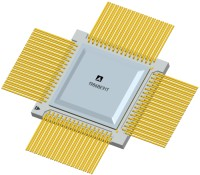
\includegraphics[width=0.3\textwidth]{fig/1986BE94.jpg}
\end{wrapfigure}

\bigskip
\begin{tabular}{l l}
Аналог & STM32F103x\ref{stm32f1}\\
ROM (Flash) & 128K \\
RAM & 32K \\
VCC & $2.2\div3.6$ V\\
Freq & 80 MHz \\
$T^o$ & $-60\div+125$\celsius \\
USB & client/host (12 MBit/s) \\
UART & 2\\
CAN & 2\\
ADC & 2x 12bit 1msps\\
DAC & 12bit\\
\end{tabular}

\bigskip

\begin{tabular}{l l l l l l l l l}
& Pins & SPI & $I^{2}C$ & ADC & DAC & CMP & extBUS &исполнение \\
\hline
1986ВЕ91Т &96 &2 &1 &16ch &2 &3 &32bit &ПЗ5,QFP\\
1986ВЕ94Т &96 &2 &1 &16ch &2 &3 &32bit &ПЗ5\\
1986ВЕ92У  &43 &2 &1 &8ch  &1 &2 &8bit &ПЗ5\\
MDR32F9Q2I &   &  &  &     &  &  &     &QFP\\
К1986ВЕ92QI &   &  &  &     &  &  &     &QFP\\
1986ВЕ93Т &30 &1 &  &4ch  &1 &2 & &ПЗ5\\
\end{tabular}

\secru{1986ВЕ4У /\cm{0}/}

32-разрядный RISC-микроконтроллер с 8-канальным 24-разрядным $\Sigma\Delta$ АЦП

\bigskip
\begin{tabular}{l l}
ROM (Flash) & 128K \\
RAM & 16K \\
VCC & $2.2\div3.6$ V\\
Freq & 36 MHz \\
$T^o$ & $-60\div+125$\celsius, К $0\div 70$\celsius\\
UART & 2\\
ADC & $\Sigma\Delta$ 24bit, 12bit \\
DAC & 12bit\\
\end{tabular}

\bigskip

\begin{tabular}{l l l l l l l l l}
& Pins & SPI & $I^{2}C$ & ADC & DAC & CMP & extBUS &исполнение \\
\hline
1986ВЕ4У &36 &1 & &8/8ch &1 & & &ПЗ5 \\
\end{tabular}

\secru{1986ВЕ1Т, К1986ВЕ1QI}

\secup

% 
% \section{NXP}
% \subsection{LPC210x}

\part{Программное обеспечение}

\chapter{Рабочая среда разработчика встраиваемых систем}


\begin{itemize}
  \item Операционная система с набором типовых утилит
  
  Для Windows требуется дополнительно установить несколько модулей из пакета
  \file{GnuWin32}, чтобы обеспечить минимальную совместимость с UNIX-средой.
  Установка \file{GnuWin32}\ описана в \labref{winsoftinstall}.
  
  Установка Linux описана в \labref{debianinstall}.
  
  \item Система управления версиями (\term{VCS})
  
  VCS предназначены для хранения полной истории изменений файлов проекта, и
  позволяют получить выгрузку проекта на любой момент времени, вести несколько
  веток разработки, получить историю изменений конкретного файла, или сравнить
  две версии файла (\term{diff}).
  
  Установка VCS \git\ описана в \labref{gitinstall}.
  
  \item Текстовый редактор или интегрированная среда разработки (IDE)
  
  Редактирование текстов программ и скриптов сборки (компиляции) с
  цветовой подсветкой синтаксиса (в зависимости от языка файла),
  \term{автодополнением}\ и вызовом программ-утилит нажатием сочетаний 
  клавиш. Также включает различные вспомогательные функции, например
  отладочный интерфейс и отображение объектов программ.
  
  Установка IDE \eclipse\ описана в \labref{eclipseinstall}.
  
  \item Тулчайн
  
  Пакет кросс-компилятора, ассемблера, линкера и других утилит типа make,
  objdump,.. для получения прошивок из исходных текстов программ.
  
  Установка GNU toolchain описана в \labref{gnuinstall}.
  
  \item ПО для программатора, JTAG-адаптера
  
  Загрузка полученной прошивки в целевое устройство, редактирование памяти, 
  внутрисхемная отладка в процессе работы устройства, прямое измение сигналов на
  выводах процессора (граничное сканирование и тестирование железа).
  
  Установка ПО для адаптеров ST-Link \labref{stlinkinst}, Segger J-Link
  \labref{jlinkinst}.
  
  \item Симулятор для отладки программ без железа
  
  Симулятор может использоваться как ограниченная замена реального железа
  для начального обучения, и для отладки программ, не завязанных на работу
  железа.
  
  Установка QEMU \labref{qemuinstall}.
  
  \item Система верстки документации
  
  Для документирования проектов и написания руководств нужна система верстки
  документации, выполняющая трансляцию текстов программ и файлов 
  документации в выходной формат, чаще всего \file{.pdf} и \file{.html}.
  
  Установка \LaTeX\ \labref{texinstall}.
  
\end{itemize}



\labpart{Установка ПО}
\labwork{Установка Debian GNU/Linux}\label{debianinstall}


\labwork{Установка Git}\label{gitinstall}

Создадим рабочий каталог, установим систему контроля версий \git\ref{git}\ и 
получим локальную копию проекта этой книги, содержащий кроме текста для издательской системы
\LaTeX\ еще и исходные коды библиотек, примеры кода и т.п., которые вы захотите
использовать в своих проектах.

\bigskip\wcmd{\url{http://git-scm.com/download/win}}

Запуститься закачка установочного пакета scm-git (\file{Git-1.9.4-preview20140611.exe}), после его загрузки
запустите установщик, 

\bigskip
\menu{Welcome>Next}

\bigskip
\menu{GNU GPL>Next} 

\bigskip
\menu{Select components>Windows Explorer Integration>Simple Context Menu>Git GUI here>Next}

\bigskip
\menu{Use Git and optional Unix tools from the Command Prompt>Next}

\bigskip
\menu{Use OpenSSH>Next}

\bigskip
\menu{Checkout Windows-style>Next}

\bigskip
\menu{Extracting files...}

\bigskip
\menu{Completing Setup>\uncheckbox\ View ReleaseNotes>Finish}

\bigskip
Проверим что \git\ правильно установился:

\bigskip\wcmd{cmd}

\bigskip
\begin{lstlisting}[style=con]
C:\Documents and Settings\pda>git --version
git version 1.9.4.msysgit.0
\end{lstlisting}

\bigskip
Первое, что вам следует сделать после установки \git а\ ---указать ваше имя и
адрес электронной почты. Это важно, потому что каждый коммит в \git е содержит
эту информацию, и она включена в коммиты, передаваемые вами:
\begin{lstlisting}[style=con]
C:\Documents and Settings\pda>git config --global user.name "Vasya Pupkin"
C:\Documents and Settings\pda>git config --global user.email no@mail.com
C:\Documents and Settings\pda>git config --global push.default simple
\end{lstlisting}

\bigskip
Эти настройки достаточно сделать только один раз, поскольку в этом случае 
\git\ будет использовать эти данные для всего, что вы делаете.
 Если для каких-то отдельных проектов вы хотите указать другое имя или
электронную почту, можно выполнить эту же команду без параметра \verb|--global|
в каталоге с нужным проектом.

\bigskip
Создаем каталог \file{D:/ARM}\ и выгружаем текущую копию этой книги из
репозитория \url{https://github.com/ponyatov/CortexMx}, создавая
свой собственный локальный \term{репозиторий проекта}.

\bigskip\wcmd{cmd}

\bigskip
\begin{lstlisting}[style=con]
C:\Documents and Settings\pda>D:
D:\>mkdir \ARM
D:\>cd \ARM
D:\ARM>git clone --depth=1 https://github.com/ponyatov/CortexMx.git book
\end{lstlisting}

\labwork{Установка GNU toolchain}\label{gnuchaininstall}


\labwork{Установка утилит GnuWin32}\label{gnuwinstall}


\labwork{Установка Java}\label{javainstall}

Для работы IDE \eclipse\ требуется установленная Java:

\bigskip\wcmd{\url{http://www.oracle.com/technetwork/java/javase/downloads/}}

\bigskip\begin{itemize}
  \item 
Минимальный вариант\ ---  ставим только Java Runtime:

\menu{Java Platform, Standard Edition>JRE>Download>Accept
License>\file{jre-8u5-windows-i586.exe}}

\menu{\file{jre-8u5-windows-i586.exe}>Welcome>\checkbox\ Change destination
folder>Install}

\menu{Destination folder>\file{D:/Java/jre8}>Next>Installing>Close}

  \item
Если вы планируете параллельно еще и осваивать язык Java\ --- ставим
Java SE JDK: 

\menu{Java Platform, Standard Edition>JDK>Download>Accept
License>\file{jdk-8u5-windows-i586.exe}}

\menu{\file{jdk-8u5-windows-i586.exe}>Welcome>Next}

\menu{Install to: \file{D:/Java/jdk8}>Next}

\menu{JRE Distination folder>Install to: \file{D:/Java/jre8}>Next}

\menu{Java SE Development Kit 8 Update 5 Successfully Installed>Close}

\end{itemize}


\labwork{Установка IDE \eclipse}\label{eclipseinstall}

\bigskip
Для работы IDE \eclipse\ требуется установленная Java \labref{javainstall}.

\bigskip
Для установки доступны два варианта:
\begin{enumerate}
\item \textbf{Eclipse Standard} базовый вариант среды, в ЛР рассмотрен именно он для иллюстрации 
ручной установки расширений
\item \textbf{Eclipse IDE for C/C++ Developers} вариант сборки 
уже включает расширение CDT, поэтому в следующий раз рекомендуем сразу качать его,
это упростит и съэкономит немного времени на установку рабочей среды
\end{enumerate}

\bigskip\wcmd{\url{http://www.eclipse.org/downloads/}}

\bigskip\menu{Eclipse Standard>Windows 32
Bit>Download>\file{eclipse-standard-luna-R-win32.zip}}

\bigskip Перетащите каталог \file{eclipse} из архива в \file{D:/ARM} и
создайте удобным для вас способом ссылку на \file{D:/ARM/eclipse/eclipse.exe}.

\bigskip
\includegraphics[height=0.3\textheight]{fig/EclipseSplash.png}

\bigskip Workspace\ --- рабочий каталог, в котором создаются каталоги отдельных
проектов, типа \file{D:/WORK}. Eclipse создаст в нем служебный каталог
\file{.metadata}, и поместит в него служебную информацию, относящуюся сразу ко
всем проектам. Как побочный эффект, если в workspace уже есть какой-то каталог,
можно создать новый проект (например \file{book}), и в левой части рабочей
области \eclipse\ в окне \window{Project Explorer}\ появится дерево файлов
\file{book/*}.

\bigskip\menu{\file{D:/ARM/eclipse/eclipse.exe}>Workspace>\file{D:/ARM}>Use as
default>OK}

\bigskip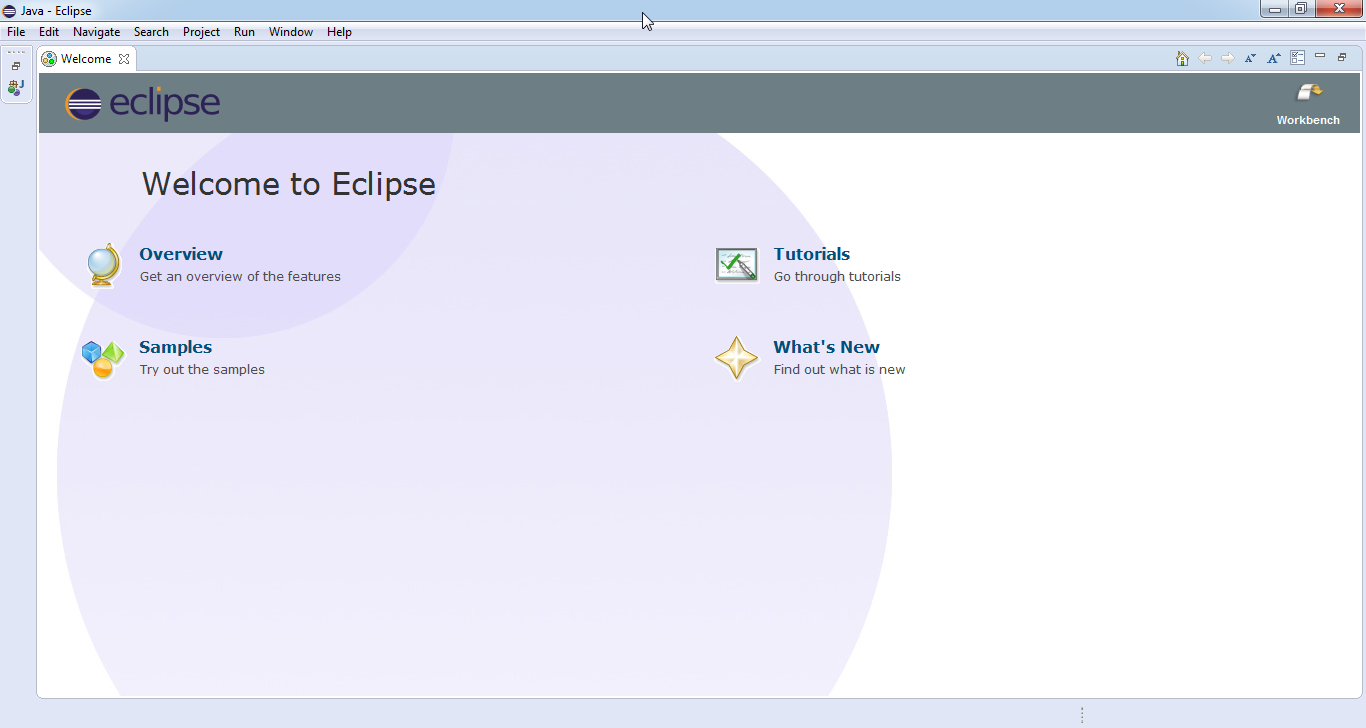
\includegraphics[width=0.9\textwidth]{fig/EclipseMain.png}

\bigskip Проверяем наличие обновлений

\bigskip\menu{Help>Check for Updates>Details>No updates found>OK}

\bigskip В базовом варианте Eclipse поддерживает только Java, поэтому нужно
установить расширение для работы с С/C++: \file{CDT}.

\bigskip
Проект \file{CDT}\ предоставляет полнофункциональную интегрированную среду
для разработки на Си и \cpp. Поддерживаются: управление проектами и
компиляцией для различных тулчейнов, стандартная сборка через
\file{make}, навигация по исходным текстам, различные инструменты для
работы с иходным текстом, такие как иерархия типов, граф вызовов, браузер
подключаемых файлов, браузер макроопределений, редактор кода с подсветкой
синтаксиса, сворачивание синтаксических структур (фолдинг) и гипертекстовая
навигация, рефакторинг и генерация кода, средства визуальной отладки,
включающие просмотр памяти, регистров и дизассемблер.

\bigskip\wcmd{\url{http://www.eclipse.org/cdt/downloads.php}}

\bigskip Выделить и скопировать в буфер обмена ссылку

\file{p2 software repository}:
\url{http://download.eclipse.org/tools/cdt/releases/8.4}.

\bigskip Добавляем сетевое хранилище пакетов для \eclipse:

\bigskip\menu{\eclipse>Help>Install New Software>Work with>Add}

\bigskip\menu{Name>CDT}

\menu{Location>http://download.eclipse.org/tools/cdt/releases/8.4}

\menu{OK}

\bigskip
Выбрать (если оно не выбралось само) хранилище \menu{Work with:>CDT},
и в дереве выбора пакетов выбрать:

\bigskip
\dirtree{%
.1 CDT.
.2 CDT Main Features.
.3 \checkbox\ C/C++ Development Tools.
.2 CDT Optional Features.
.3 \checkbox\ C/C++ C99 LR Parser.
.3 \checkbox\ C/C++ GCC Cross Compiler Support.
.3 \checkbox\ C/C++ GDB Hardware Debugging.
}

\bigskip
\menu{Next>Next>Licenses>Accept>Finish}

\bigskip После установки пакетов появится окно с запросом перезапуска \eclipse.

\bigskip Аналогично ставим плагин GNU ARM Eclipse:

\bigskip
\menu{Help>Install>Work with>Add}

\menu{Name>GNU ARM plugin}

\menu{Location>\url{http://sourceforge.net/projects/gnuarmeclipse/files/Eclipse/updates/}}

\dirtree{%}
.1 GNU ARM C/C++ Cross Development Tools.
.2 \checkbox\ Cross Compiler Support.
.2 \checkbox\ Generic Cortex-M Project Template.
.2 \checkbox\ STM32Fx Project Templates.
.2 \checkbox\ OpenOCD Debugging Support.
}

\menu{Warning: You install unsigned content>Ok}

\bigskip
В \eclipse\ есть так называемые \term{перспективы} (perspective)\ --- это
переключаемые режимы отображения рабочего набора окон, настроенные под тип
работы. По умолчанию запускается перспектива \window{Java}. Нас
интересует перспектива \window{C/C++}:

\bigskip\menu{Window>Open Perspective>Other>C/C++>Ok}

\bigskip Также перспективу можно переключить кнопкой на панели в правом верхнем
углу:

\bigskip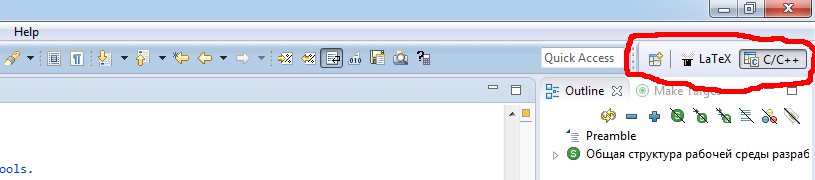
\includegraphics[width=0.9\textwidth]{fig/eclperpective.png}

\bigskip Для настройки привычных вам клавиш можно сразу зайти в
глобальные настроки среды и поменять привязку клавиш:

\bigskip\menu{Window>Preferences>General>Keys}

\menu{Type filter here:>F12}

\menu{Command}

\menu{Activate Editor>Binding>/удалить/}

\menu{Build Project>Binding>/нажать \keys{F12}/}

\menu{Apply>OK}



\labwork{Установка симулятора QEMU}\label{qemuinstall}

Нередко в практике разработчика возникают ситуации, когда программное обеспечение (ПО) для микроконтроллера
приходится писать в отсутствии под рукой аппаратной платформы.

Например, печатная плата устройства отдана на подготовку к производству, а времени ждать
готовое устройство для тестирования на нем программного обеспечения нет.

В таких случаях для оценки работоспособности ПО можно воспользоваться программным симулятором целевого микроконтроллера.

Для интегрированной среды разработки \eclipse\ CDT в качестве программного
симулятора микроконтроллеров ARM можно использовать симулятор (или виртуальную машину,если быть точным) 
\file{qemu-arm} с интерфейсом командной строки:

\bigskip\menu{\wcmd{\url{http://qemu.weilnetz.de/w32/}}>\file{qemu-w32-setup-20140702.exe}}

\menu{\file{qemu-w32-setup-20140702.exe}>Welcome>Next>License>Agree}

\menu{Choose Components}

\dirtree{%
.1 QEMU.
.2 \uncheckbox\ System Emulations.
.3 \checkbox\ arm.
.3 \checkbox\ armw.
}

\menu{Next}

\menu{Destination Folder>\file{D:/ARM/qemu}>Next>Finish}

\bigskip Добавьте \file{D:/ARM/qemu}\ в системную переменную
\file{\$PATH}\ (\labref{winpath}).

\bigskip

\begin{lstlisting}[style=con]
C:\Documents and Settings\pda>qemu-system-arm -version
C:\Documents and Settings\pda>cat D:\ARM\qemu\stdout.txt
QEMU emulator version 2.0.90, Copyright (c) 2003-2008 Fabrice Bellard
\end{lstlisting}


\labwork{Установка ПО ST-Link для \vld}\label{labinststsoft}

\menu{\wcmd{\url{http://www.google.com}}>ST-Link>ST-Link - STMicroelectronics}

\bigskip
\begin{tabular}{l l l}
\menu{STSW-LINK002>Download}	&ST-LINK USB driver for Windows XP&драйвер\\
\menu{STSW-LINK004>Download}	&STM32 ST-LINK utility&ПО программатора\\
\end{tabular}

\bigskip
\menu{\file{st-link\_usbdriver.zip}>\file{ST-Link\_USBdriver.exe}}

\menu{STLinkDriver>Welcome>Next>Install
to>\file{C:/ARM/STM32/STdriver}>Next>Install>Finish}

\bigskip
\menu{\file{stsw-link004.zip}>\file{STM32 ST-LINK Utility\_v3.4.0.exe}}

\menu{ST-LINK
Utility>Next>License>Yes>Distination>\file{C:/ARM/STM32/STLinkUtil}>Finish}

\menu{(сам запустился) Device Driver Install Wizard>Далее>Установить}

\bigskip
\menu{\winstart>STMicroelectronics>ST-LINK Utility>STM32 ST-Link}

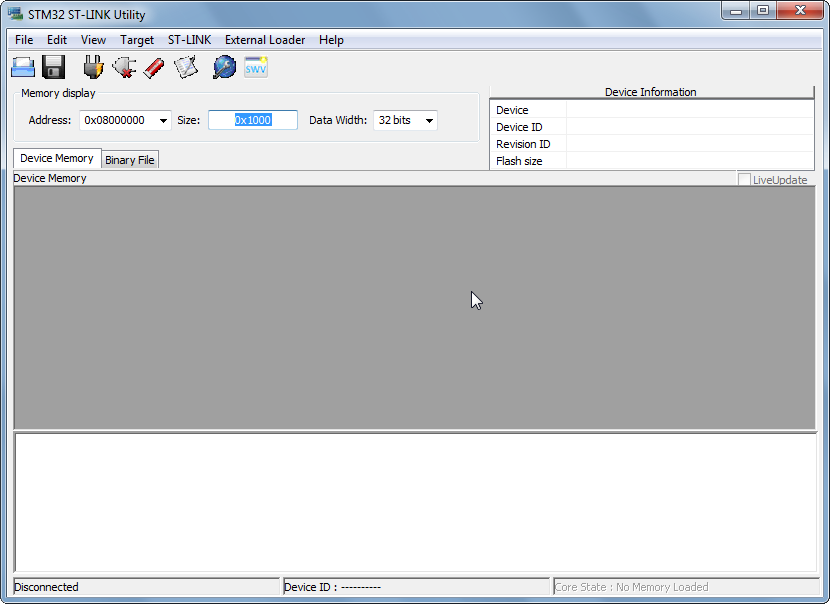
\includegraphics[height=0.5\textheight]{fig/stlink0.png}

\bigskip
\menu{STutil>Target>Connect}

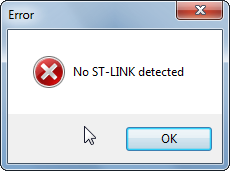
\includegraphics[height=0.2\textheight]{fig/nostlink.png}

\bigskip
Подключаем плату \vld\ кабелем, в системе подключается новое устройство,
на плате запускается ранее залитая в МК прошивка:

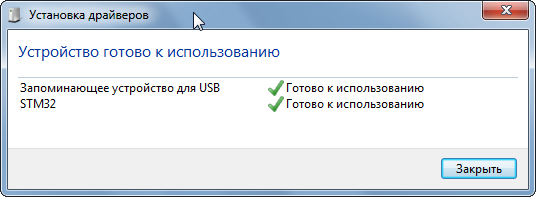
\includegraphics[height=0.3\textheight]{fig/stdrvok.png}

\bigskip
\menu{STutil>Target>Connect}

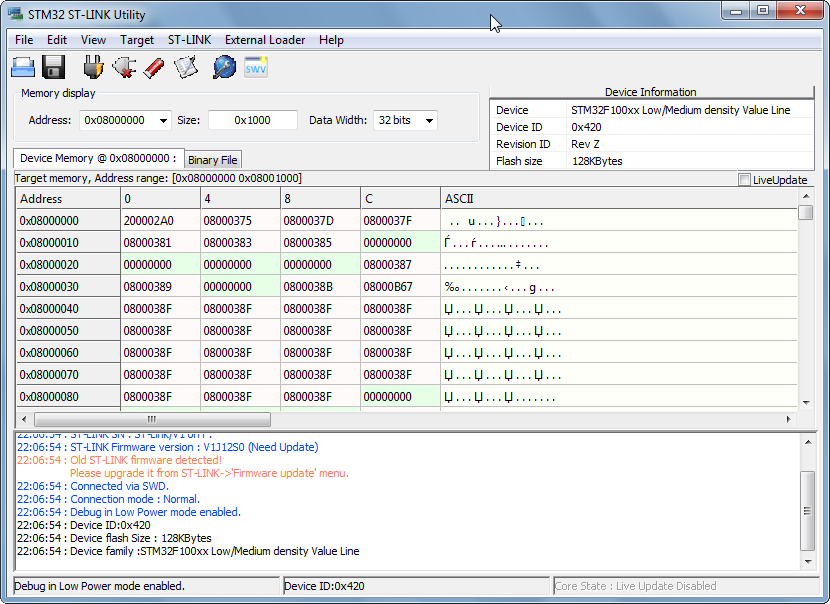
\includegraphics[width=0.9\textwidth]{fig/stconnected.png}

\bigskip
Обновление прошивки ST-Link:

\menu{ST Link>ST-LINK>Firmware update>Device Connect>not in DFU
mode}

\menu{передергиваем плату>Device connect>Upgrade to V.1.J13.S0>Yes}

\bigskip



\labwork{Установка системы верстки документации \LaTeX}\label{texinstall}

Если вы планируете писать полноценную документацию на программы
и оборудование, или участовать в доделке этой книги, вы можете установить
систему верстки \LaTeX.

Для работы с \TeX\ требуется довольно приличное по усилиям
(само)обучение \cite{lvovsky}, но оно оправдывается если вы часто 
пишете документацию, особенно если в ней больше 10 формул.
Готовить документацию в M\$\ Word\ --- (само)убийство мозга и времени,
идеология подстановочных макросов \TeX, богатый набор доп.пакетов
и командный ввод формул очень доставляют.

\win{Скачайте и установите пакет \miktex:}

\bigskip\wcmd{\url{http://miktex.org/download}>Other Downloads>Net Installer}

\menu{Save as:>\file{D:/ARM/soft/MikTeX/miktex-netsetup-2.9.4503}}

\bigskip Загрузка дистрибутивных файлов

\menu{\file{miktex-netsetup-2.9.4503}>License>Accept>Далее}

\menu{Task>Download>Далее}

Если у вас постоянное internet-соединение: \menu{Package Set>Basic MiKTeX>Далее}

Для offline работы\footnote{когда неизвестно какие пакеты понадобятся\ ---
\miktex\ умеет их докачивать по необходимости} \menu{Package
Set>Complete MikTeX>Далее}

\menu{Download Source>Russian Federation (ctan.uni-altai.ru)>Далее}

\menu{Distribution
Directory>\file{D:/ARM/soft/MikTeX}>Далее>Start>Executing>Далее>Close}

\bigskip Установка из ранее загруженного дистрибутива

\menu{\file{D:/ARM/soft/MikTeX/miktex-\alarm{netsetup}-2.9.4503}>License>Accept>Далее}

\menu{Task>Install>Далее>Basic MiKTeX>Далее}

\menu{Install for>Anyone/Only for user>Далее}

\menu{Install \alarm{from}:>\file{D:/ARM/soft/MikTeX}>Далее}

\menu{Install to:>\file{D:/LaTeX/MiKTeX}>Далее}

\menu{Settings}

\menu{Preferred paper>A4}

Важная опция: автоматическая докачка отсутствующих пакетов
\alarm{\menu{Install missing packages>Yes}}

\menu{Далее>Start>Executing>Close}

\bigskip Двухступенчатая установка позволяет сначала скачать полный дистрибутив
\miktex, а затем установить его на другой компьютер, не подключенный к
\internet, или c медленным/платным каналом не дающим взять и качнуть 200 Мб.

\bigskip Для удобной работы с \file{.tex} файлами в \eclipse\ нужно поставить 
дополнение \file{TeXlipse}:

\bigskip
\menu{\eclipse>Help>Install>Work with>Add}

\menu{Name>TeXlipse}

\menu{Location>\url{http://texlipse.sourceforge.net}}

\dirtree{%}
.1 TeXlipse.
.2 \checkbox\ TeXlipse.
}

%\include{ПО для JTAG-адаптера}

\chapter{Первые шаги}
\labpart{Первые шаги}
\labwork{Создание нового проекта в \eclipse}\label{labecreprj}

Создадим новый проект, напишем простую программу, и запустим ее в отладчике.

\bigskip\menu{\eclipse>File>New>Project>C/C++>C Project>Next}

\menu{Project name>hello}

\menu{Project type>Makefile project>Empty project}

\menu{Toolchains>Cross ARM GCC}

\menu{Finish}

\menu{This kind of project associated with C/C++ perspective>Yes}

\labwork{Создание Makefile}\label{labmkmake}

Стоит объяснить, почему при создании проекта мы выбрали тип \file{Makefile
project}, хотя были доступны более логичные варианты типа \file{ARM C Project}.

Утилита \make\ ведет свою историю с 70х гг. Компьютеры тогда были большими,
тяжелыми, а главное медленными и с очень маленькой памятью (десятки$\div$сотни
Кб).
Компиляторам зачастую не хватало памяти, чтобы скомпилировать большую программу.
Кроме того, скорость их запуска и работы была тоже черепашьей.
Поэтому исходный код программы делили на модули, компилировали или
ассемблировали каждый модуль по-отдельности в \term{объектный код}, а затем уже
на конечном этапе с помощью \term{линкера}\ собирали несколько файлов объектного
кода в один исполнямый файл.

Для ускорения и упрощения этого процесса и была создана утилита \make.
Чтобы не вызывать лишний раз компилятор или какой-нибудь транслятор, в файле
\makefile\ прописываются зависимости между файлами. Затем запускается \make\ c
указанием какой файл нам нужно получить, и выполняется цепочка вызовов
нужных программ.

Следует отметить, что утилита \make\ используется до сих пор для сборки самых
современных программных пакетов (типа GCC 4.9.x), правда в комплексе с другими
средствами, обеспечивающими переносимость программ между разными ОС и
автогенерацией зависимостей из исходного кода.

\bigskip
Для наших целей \make\ используется как самое простое средство управления
компиляцией проекта. В средах разработки, особенно в коммерческих,
используются служебные файлы проектов, иногда бинарные, чаще текстовые, но
всегда запутанные и весьма развесистые.

Если вам вдруг понадобится откомпилировать ваш проект на другом компьютере,
с другой архитектурой, возможно вообще без графического
интерфейса\footnote{например какой-нибудь удаленный сервер на
процессоре 1995ВМ666 под раскряченным Solaris 7$\alpha$4, на котором лежит
криптобиблиотека, использующая при компиляции трофейный электро-механический 
энкодер, существующий в единственном экземпляре \smiley}, или вы вдруг решите
попробовать работать в другой IDE\ --- вы тут же вляпаетесь в ситуацию, 
когда нечем открыть файл проекта с заботливо прописанными опциями
компиляции.

\bigskip
\menu{\eclipse>\window{Project Explorer}>\file{hello}>\rms>Open Project}

\menu{\eclipse>\window{Project Explorer}>\file{hello}>\rms>New>File>File
name:>\file{Makefile}}

\bigskip
\lstinputlisting[style=mk,inputencoding=cp1251]{tmp/hello.mk}

\bigskip
Этот пример \makefile\ достаточно универсален и самодостаточен для большинства
проектов в этой книге. Кажущийся большой объем получился за счет использования
комментариев и переменных. И те, и другие служат для документирования проекта,
и повышают читаемость кода. В принципе никто не мешает\footnote{особенно для
микроскопических объемов исходных текстов программ для контроллеров\ ---
в самом худшем случае какие-то жалкие сотни Кб}\ написать несколько строк в
\file{.bat}нике с явным указанием опций компиляторам, или вообще откомпилировать
все исходники сразу одним вызовом \file{gcc}\ с кучей опций и списком исходных
файлов. Но если вам потребуется что-то изменить, куда проще и быстрее сделать
это в аккуратно оформленном самодокументированном \makefile.



\labwork{Hello World}\label{labhello}

Для начала нужно рассмотреть набор файлов минимального проекта:

\begin{itemize}

\item \file{README.txt}

Краткая информация о проекте\ --- название, авторы, обязательно ссылки на
\git-репозиторий, сайт, форум, и т.п.
 
\item \file{Makefile}

Файл с описанием зависимостей между файлами, настройками проекта (в переменных)
и правилами вызова компиляторов.

\item \file{startup.S}

Стартовый код процессора, включает инициализацию системы тактирования, мапинга
памяти, контроллера прерываний и минимальную инциализацию периферии.
Пишется на ассемблере, т.к. на Си получается слишком сложно, синтаксически
запутанно, или очень специфично для компилятора.

\item \file{startup.c}

Сишный вариант стартового кода, использование синтаксических ухищрений
GNU CC позволяет обойтись без ассемблера даже для описания таблицы векторов,
но для начинающего сложновато разобраться.

\item \file{init.c}

Сишный код инициализации железа (синтаксически легче описать блоки кода,
зависимые от целевого процессора).

\item \file{main.c}

Основной код, решающий поставленную задачу. 

\item \file{\$CPU.ld}

Скрипт линкера, настраивающий генерацию выходного бинарного файла в 
зависимости от целевого процессора\ --- прежде всего организация памяти,
и размещение сегментов кода/данных по фактическим адресам памяти.
Поэтому здесь имя файла задано через переменную, описанную в \makefile.

\item \file{generic.ld}

Скрипт линкера, содержащий общую часть для всех микроконтроллеров

\end{itemize}

\bigskip Создаем эти файлы аналогично \makefile\ в \labref{labmkmake}:

\bigskip\menu{\eclipse>\window{Project Explorer}>\file{hello}>\rms>New>File>File
name:>\file{НужныйФайл.xxx}}

\lstinputlisting[inputencoding=cp1251,title=README.txt]{hello/README.txt}

\lstinputlisting[style=asm,inputencoding=cp1251,title=startup.S]{hello/startup.S}

\lstinputlisting[style=cpp,inputencoding=cp1251,title=init.c]{hello/init.c}

\lstinputlisting[style=cpp,inputencoding=cp1251,title=main.c]{hello/main.c}

\lstinputlisting[style=gnuld,inputencoding=cp1251,title=arm7tdmi.ld]{hello/arm7tdmi.ld}

\labwork{Настройка отладчика в \eclipse}\label{labgdbinst}

\cp{http://makesystem.net/?p=2146}

 На сегодняшний день существуют много способов и инструментов для отладки
 embedded приложений, начиная с отладки “в железе” (внутрисхемная отладка)  и
 заканчивая всякими симуляторами. У каждого метода есть свои плюсы и минусы, но
 поскольку мы будим писать приложения для реальных устройств, то
 предпочтительней реальная отладка (в железе), то есть приложение будит
 исполняться непосредственно микроконтроллером.
 
Что нам понадобится для “железной отладки” :

\begin{itemize}
  \item 
ARM микроконтроллер (для симуляции необязателен)
  \item 
JTAG/SWD адаптер (для симуляции необязателен)
  \item 
GDB сервер (транслятор интерфейсов GDB/JTAG)
  \item 
GDB отладчик (имеет встроенный симулятор ARM7TDMI, используется для первых лаб) 
  \item 
плагин C/C++ GDB Hardware Debugging 
  \item 
плагин Eclipse Embedded Systems Register View 
\end{itemize}

\term{JTAG адаптер}\ (он же \term{программатор}) следует выбрать тот, который
поддерживает именно ваш микроконтроллер, а еще лучше, микроконтроллеры разных
производителей.
В моем случае (еще с давних времен у меня завалялись кристаллы от Texas
Instruments, ST Microelectronics, NXP, Atmel, Cypress), я сразу решил найти
программатор поддерживающий имеющиеся у меня камни. Порыскав в интернетах, мой
выбор пал на китайский клон знаменитого J-Link, в добавок к которому идет уйма
полезных утилит от Segger Microcontroller (тут обошлось без китая \smiley),
облегчающие жизнь разработчику.

В этой книге также рассмотрено несколько простых варинтов JTAG-адаптеров,
которые вы можете сделать сами, не обладая выдающимися знаниями в электронике
и технологиях производства печатных плат.

\bigskip
Структура аппаратно-программного комплекта для отладки:

\menu{микроконтроллер>JTAG/SWD>адаптер>LPT/USB>GDB сервер>протокол
GDB>GDB отладчик>IDE}

Адаптер подключается к выводам МК с помощью колодки (JTAG) или гребенки (SWD).

К компьютеру адаптер подключается через однин из распространенных интерфейсов:
совсем дешевые варинты ``на пяти резисторах'' через порт LPT, чуть подороже
через USB, совсем дорогие проф.модели могут иметь Ethernet интерфейс.

\bigskip
\term{Отладчик}\ (дебаггер, англ. debugger)\ --- компьютерная программа,
предназначенная для поиска ошибок в других программах. Отладчик позволяет
выполнять пошаговую трассировку, отслеживать, устанавливать или изменять
значения переменных в процессе выполнения кода, устанавливать и удалять
контрольные точки или условия остановки, сопоставлять двоичный код\ --- eгo
исходному тексту (на основе которых можно точно определить выполняемые
программой действия) и т.д. (Wiki)

Практически во все тулчейны входит утилита GDB (\file{arm-none-eabi-gdb}), это и
есть отладчик GNU. В принципе, дебаггер выполняет два типа действий:
управление исполнением программы в кристалле (через отладочный интерфейс) и
вывод результатов в консоль/графическую оболочку.

\bigskip
При сборке тулчайна (из исходников) невозможно заранее сказать, какой набор
отладочных средств будет у конечного пользователя\ --- у типичного
ембеддера\footnote{разработчика ПО под встраиваемые системы}\ запросто наберется
пара-тройка различных \jtag-адаптеровв, несколько демоплат со
встроенным адаптером, причем с разными процессорами, несколько собственных
устройств с самодельными отладочными интерфейсами, и еще для комплекта пару
чисто программных симуляторов \arm-ядер.

Задачу унификации интерфесов, и подключения всего этого зоопарка к одному и тому
же отладчику \gdb\ выполняет \term{\gdb-сервер}. Отладчик общается с сервером по
одному и тому же унифицированному \term{\gdb-протоколу}\ через последовательный
порт или TCP/IP соединение, а все сложности взаимодействия с железом берет на
себя сервер.
Это сделано (в том числе) для тех случаев, когда \gdb-отладчик работает на одном
ПК а \gdb-сервер на другом (в соседней комнате или соседнем государстве
\smiley). Опять же, сервер надо выбрать тот, который поддерживает ваш
\jtag-адапер или эмулятор.

\bigskip
\gdb, как и все остальные утилиты тулчайна, работает из командной строки, что
не всем удобно \smiley, поэтому для начала стоит научиться им пользоваться из
графической оболочки. \eclipse\ как и подобает серьёзной IDE, имеет средства
работы с \gdb, заменяющие его консоль, имеет графические кнопки для вызова
всех отладочных команд, и отображает содержимое регистров, памяти и т.п. в
графических окнах. Взаимодействие \eclipse/\gdb\ обеспечивает плагин \file{C/C++
GDB Hardware Debugging}, входящий в состав уже установленного ранее
расширения \file{CDT}.

\bigskip
Проверить наличие плагина можно так:

\menu{Help>Install New Software>Work with:>All Available Sites}

\menu{\uncheckbox\ Hide items that are already installes}

\menu{type filter>GDB}

\dirtree{%
.1 GDB.
.2 CDT Optional Features.
.3 \checkbox\ C/C++ GDB Hardware Debugging.
.2 Mobile and Device Development.
.3 \checkbox\ C/C++ GDB Hardware Debugging.
}

\bigskip

Прежде всего отключим оптимизацию кода проекта, задав в
\makefile\ значение переменной \file{OPTFLAGS = -O0}. 

Затем, нужно включить в проекте генерацию отладочной информации\footnote{имена
переменных, функций и т.п. объектов программы, в т.ч. и сами строки исходного
кода}, добавив опцию \file{-g[N]}.

Существуют три уровня отладочной информации:

\begin{enumerate}
\item в объектный код вставляется минимальный объем отладочной информации. Ее
вполне достаточно для трассировки вызовов функций и исследования глобальных
переменных, тем не менее, отсутствует информация для сопоставления выполняемого
кода со строками исходного кода и информация для отслеживания локальных
переменных.

\item используется по умолчанию. Помимо всей отладочной информации пepвoгo
уровня он дополнительно включает данные, необходимые для сопоставления строк
исходного кода с выполняемым кодом, а также имена и расположение локальных
переменных.

\item помимо всей отладочной информации пepвoгo и второго уровней, включает
дополнительную информацию, в частности определения макросов препроцессора.
\end{enumerate}

Используем 3 уровень, изменив в \makefile\ значение переменной 
\file{DEBFLAGS = -g3 -ggdb}. Опция \term{-ggdb}\ задает дополительно формат
отладочной информации. Доступны форматы STABS, DWARF2 и родной формат платформы.

В файле \file{startup.o.dump}\ при этом появляются дополнительные секции
с отладочной информацией, и в заголовок добавляются флаги, указывающие на
ее наличие:

%\lstinputlisting[style=objdump,title=startup.o.objdump]{hello/startup.o.objdump}
\begin{lstlisting}[style=objdump,title=startup.o.objdump]
startup.o:     file format elf32-littlearm
architecture: armv4t, flags 0x00000011: HAS_RELOC, HAS_SYMS
...
  4 .debug_line   00000044  00000000  00000000  000000b0  2**0
                  CONTENTS, RELOC, READONLY, DEBUGGING
  5 .debug_info   00000044  00000000  00000000  000000f4  2**0
                  CONTENTS, RELOC, READONLY, DEBUGGING
  6 .debug_abbrev 00000014  00000000  00000000  00000138  2**0
                  CONTENTS, READONLY, DEBUGGING
  7 .debug_aranges 00000020  00000000  00000000  00000150  2**3
                  CONTENTS, RELOC, READONLY, DEBUGGING
\end{lstlisting}   

\bigskip
Для настройки отладочного интерфейса заходим в меню

\menu{Run>Debug Configurations\ldots}

\menu{GDB Hardware Debugging>\rms>New}

В результате открывается окно с настройками отладки.

\bigskip
Для начала попробуем работу нашей прошивки на встроенном в \gdb\ программном
симуляторе процессора \file{ARM7TDMI}.

\bigskip
Вкладка Main.

\bigskip
В поле Name, можно дать имя всей конфигурации отладки, поскольку даже для одного
проекта бывают разные конфигурации отладки (скажем для отладки в RAM или Flash
памяти).

\menu{Name:>ARM7TDMI simulator}

В поле Project указываем имя проекта (поскольку в нашем workspace может быть
более одного проекта)

\menu{Project:>hello}

В поле C/C++ Application указываем имя *.elf файла сгенерированного после
компиляции (с введенными ранее настройками для Debug прошивки) проекта и который
будет использован во время отладки.

\menu{C/C++ Application:>startup.o}

\alarm{Перед тем как перейти к следующей вкладке, в нижней части окна
обязательно выбираем}

\menu{Legacy GDB Hardware Debugging Launcher}

\menu{Apply}

\bigskip
Вкладка Debugger. Здесь мы установим связь между отладчиком и графической
оболочкой, а также между отладчиком и \gdb-сервером (отсюда и название вкладки).

\bigskip
В поле GDB Command указываем имя отладчика из тулчайна.
Должен быть прописан в \file{\$PATH}, или можно указать полный путь

\menu{GDB Command:>arm-none-eabi-gdb}

В соответствии с идеологией ведущих разработчиков Free Software Foundation,
\gdb\ вместо собственного графического пользовательского интерфейса
предоставляет возможность подключения к внешним IDE, управляющим графическим
оболочкам либо использовать стандартный консольный текстовый интерфейс” (Wiki).
В общем, mi (Machine Interface) это протокол общения между отладчиком и
графической оболочкой.

\menu{Command Set:>Standard (Windows)}

\menu{Protocol Version:>mi}

Как ранее было сказано, общение между отладчиком и сервером осуществляется через
последовательный или TCP/IP порт, поэтому в общем случае следует выбирать опции
типа:

\menu{Remote Target>\checkbox\ Use remote target}

\menu{JTAG Device:>Generic TCP/IP}

\menu{IP address:>localhost}

\menu{Port number:>12345}

\alarm{Но поскольку мы собираемся использовать встроенный симулятор ARM7,
пока нужно \textbf{выключить} удаленную отладку:}

\menu{\uncheckbox\ Use remote target}

\bigskip

\menu{Apply}

\bigskip
Вкладка Startup (предписания отладчику перед началом работы).

\bigskip
Сброс необходим для того чтобы очистить регистры ARM процессора от значений
полученных в ходе предыдущей отладки (по желанию)

\menu{Reset and Delay (seconds):>3}

Останавливаем процессор для настройки эмулятора и загрузки отлаживаемой прошивки

\menu{\checkbox\ Halt}

В (пустом) текстовом поле вводим команды, выполняемые при старте отладки.

\bigskip
Настало время вернутся к вопросу об использовании симуляции микроконтроллеров
\file{ARM7TDMI}. На самом деле с этой задачей запросто справляется сам \gdb,
если указать ему стартовые команды:

\menu{target sim}

\menu{load}

%monitor speed auto
%monitor endian little
%monitor flash device = STM32F103RB
%monitor flash download = 1
%monitor flash breakpoints = 1

Из какого файла грузить прошивку

\menu{Load image>Use project binary}

Из какого файла грузить отладочную информацию\footnote{можно использовать
отдельный \file{.sym} файл}

\menu{Load symbols>Use project binary}

\menu{Apply}

\bigskip
Вкладка Common

\bigskip

\menu{Display in favorites menu>\checkbox\ Debug}

\menu{Standard Input and Output>\checkbox\ Allocate console}

\menu{\checkbox\ Launch in background}

\menu{Apply}

% \bigskip
% Задача \gdb-сервера слушать последовательный или TCP/IP порт и перенаправлять
% команды \jtag-адаптеру, а он в свою очередь микроконтроллеру.
% 
% Поскольку мы уже указали отладчику использовать локальный TCP/IP порт
% \file{localhost:12345}, осталось указать серверу какой отладочный интерфейс
% использовать.

\bigskip
При первом запуске отладки, \eclipse\ просит разрешение на переход в режим
отображения отладки (Debug perspective). Разрешаем и ставим галку “\checkbox\
больше не спрашивать“. Далее, открывается отображение многочисленных окон,
каждое со своим предназначением (окна исходного кода, окно дизассемблера, окно
отображения памяти и т.д.). При желании можно добавить различные окна через меню
\menu{Window>Show View}.

\bigskip

Первый запуск отладчика \bug: \menu{кнопка клопа>ARM7TDMI simulator}

Последующие запуски (последнего) отладчика: просто \keys{F11} 

\bigskip
\begin{lstlisting}
symbol-file C:\\ARM\\book\\hello\\startup.o
Reading symbols from C:\ARM\book\hello\startup.o...done.
target sim
load C:\\ARM\\book\\hello\\startup.o 
Connected to the simulator.
Loading section .text, size 0x50 vma 0x0
Start address 0x0
Transfer rate: 640 bits in <1 sec.
\end{lstlisting}


\chapter{Система управления версиями Git}
\chapter{Управление версиями при написании ПО}

\section{Git}\label{git}\cite{progit}



\chapter{Интегрированная среда разработки \eclipse}
\secru{\eclipse}

Например нажатием \keys{F3}\ в \eclipse\ можно переместится на
  определение функции, на имени которой находится текствый курсор.
  
    Автодополнение\ --- редактор предлагает варианты полного написания
  идентификаторов и ключевых слов по первым буквам и нажатию обычно
  \keys{Ctrl+Tab} или \keys{Ctrl+N}. Также автоматически расставляются
  закрывающие скобки, закрывающие операторы управляющих структур типа begin/end,
  и генерируются синтаксические элементы циклов при вводе ключевых слов
  if/for/while. Особенно удобно автодополнение при написании кода на ООП 
  языках\  --- при вводе имени класса или объекта и точки предлагается меню с
  именами данных и методов класса. 
  
  При вводе имени функции и скобки выводится всплывающее окно с подсказкой\ ---
  определение функции с типом возвращаемого значения, типом и именами
  параметров.
  
  Интерфейс IDE часто предусматривает различные вспомогательные окна,
  показывающие имена и свойства объектов, описанных в программе (переменные,
  функции, структуры,..), структуру проекта с зависимостями между файлами, блоки
  справки в зависимости от текущего выделенного элемента и т.п.
  
  Часто IDE имеет встроенный графический интерфейс для отладки программ,
  используя для этого интерфейсные библиотеки для программатора и
  специальный отладочный код, добавляемый к вашей программе при
  компиляции. Используя аппаратный модуль отладки на целевом процессоре и
  отладочный код, IDE обеспечивает отображение значений и изменений регистров
  процессора, состояние переферии, позволяет задать точки останова в программном
  коде, в т.ч. условные по значению или измениею переменных или регистров
  железа.
  При использовании ОС реального времени и системы аппаратной многозадачности
  отображается загрузка ядер, загрузка процессора и используемые ресурсы для
  каждой задачи, работа планировщика, и т.п.
  
Для удобной работы доступно несколько бесплатных вариантов IDE, далее
рассмотрим два варианта: тяжелая суперуниверсальная среда \eclipse, и легкая 
в отношении требуемых ресурсов системы CodeLite.
  


\chapter{Пакет кросс-компиляции GNU toolchain}

  Компилятор преобразует программы на языке программирования в \term{объектный
  код} (смесь кусочков машинного кода со служебной информацией) или в
  текст на языке ассемблера.
  
  \term{Кросс-компилятор}\ (arm-none-eabi-gcc) отличается от обычного
  компилятора тем, что генерирует код не для компьютера на котором он выполняется
  (\term{хост-система}, \verb|$HOST|), а для компьютера другой
  архитектуры\ --- \term{целевой} системы, \verb|$TARGET|.
  
  \term{Ассемблер}\ (as) преобразует человекочитаемый код программы в объектный
  код.
  
  \term{Линкер}\ (ld) объединяет несколько файлов объектного кода в один,
  и корректирует машинный код с учетом его конечного размещения в памяти
  целевой системы (адреса переменных, адреса переходов, размещение сегментов
  кода и данных в физической памяти целевой системы).
  
  \term{Дампер}\ (objdump) преобразует сегменты кода/данных из файла,
  полученного линкером, в формат, необходимый для ПО программатора: бинарные файлы, Intel
  HEX, ELF,.. загружаемые в масочное ПЗУ, FlashPROM (и EEPROM данных на МК
  ATmega).
  


\part{Отладка}

% \chapter{Рабочая среда разработчика встраиваемых систем}


\begin{itemize}
  \item Операционная система с набором типовых утилит
  
  Для Windows требуется дополнительно установить несколько модулей из пакета
  \file{GnuWin32}, чтобы обеспечить минимальную совместимость с UNIX-средой.
  Установка \file{GnuWin32}\ описана в \labref{winsoftinstall}.
  
  Установка Linux описана в \labref{debianinstall}.
  
  \item Система управления версиями (\term{VCS})
  
  VCS предназначены для хранения полной истории изменений файлов проекта, и
  позволяют получить выгрузку проекта на любой момент времени, вести несколько
  веток разработки, получить историю изменений конкретного файла, или сравнить
  две версии файла (\term{diff}).
  
  Установка VCS \git\ описана в \labref{gitinstall}.
  
  \item Текстовый редактор или интегрированная среда разработки (IDE)
  
  Редактирование текстов программ и скриптов сборки (компиляции) с
  цветовой подсветкой синтаксиса (в зависимости от языка файла),
  \term{автодополнением}\ и вызовом программ-утилит нажатием сочетаний 
  клавиш. Также включает различные вспомогательные функции, например
  отладочный интерфейс и отображение объектов программ.
  
  Установка IDE \eclipse\ описана в \labref{eclipseinstall}.
  
  \item Тулчайн
  
  Пакет кросс-компилятора, ассемблера, линкера и других утилит типа make,
  objdump,.. для получения прошивок из исходных текстов программ.
  
  Установка GNU toolchain описана в \labref{gnuinstall}.
  
  \item ПО для программатора, JTAG-адаптера
  
  Загрузка полученной прошивки в целевое устройство, редактирование памяти, 
  внутрисхемная отладка в процессе работы устройства, прямое измение сигналов на
  выводах процессора (граничное сканирование и тестирование железа).
  
  Установка ПО для адаптеров ST-Link \labref{stlinkinst}, Segger J-Link
  \labref{jlinkinst}.
  
  \item Симулятор для отладки программ без железа
  
  Симулятор может использоваться как ограниченная замена реального железа
  для начального обучения, и для отладки программ, не завязанных на работу
  железа.
  
  Установка QEMU \labref{qemuinstall}.
  
  \item Система верстки документации
  
  Для документирования проектов и написания руководств нужна система верстки
  документации, выполняющая трансляцию текстов программ и файлов 
  документации в выходной формат, чаще всего \file{.pdf} и \file{.html}.
  
  Установка \LaTeX\ \labref{texinstall}.
  
\end{itemize}



\labpart{Установка ПО}

\section{Выбор и установка операционной системы}

\subsection{MacOS}

Этот странный пока случай не рассматриваем\ --- у меня нет под рукой Мака \smiley.

\subsection{Windows}

Самый распространенный вариант. Вам придется ограничиться этим вариантом если вам не повезло
с поставщиком контроллера: windows-only ПО поддержки, например софт для программатора, или
внезапно библиотеки только для коммерческих компиляторов. Аналогичная ситуация будет в случае
покупки какого-нибудь специфичного оборудования (лог.анализатор, измерительное 
оборудование или просто принтер).

Установку ОС не рассматриваем.

\win{Секции текста книги, зависящие от ОС, будут выделены вот так.}

Для разработки встраиваемого ПО нужно поставить несколько пакетов, обеспечивающих
совместимость с UNIX средами \ref{winsoftinstall}.

\subsection{Linux}\label{linux}

\begin{enumerate}
\item \label{linuxref1}\linux\ удобен для разработчика, 
\item Если он вам не удобен, см п.\ref{linuxref1}
\end{enumerate}

\lin{Секции текста книги, зависящие от ОС, будут выделены вот так.}

\lin{\labwork{Установка Debian GNU/Linux}\label{debianinstall}}

\section{Установка инструментального программного обеспечения}

\win{\labwork{Установка инструментального ПО для Windows}\label{winsoftinstall}}

Создадим рабочий каталог, установим систему контроля версий \git\ref{git}\ и 
получим локальную копию проекта этой книги, содержащий кроме текста для издательской системы
\LaTeX\ еще и исходные коды библиотек, примеры кода и т.п., которые вы захотите
использовать в своих проектах.

%\labsection{Установка Git}\label{gitinstall}

\bigskip\wcmd{\url{http://git-scm.com/download/win}}

Запуститься закачка установочного пакета scm-git (\file{Git-1.9.4-preview20140611.exe}), после его загрузки
запустите установщик, 

\bigskip
\menu{Welcome>Next}

\bigskip
\menu{GNU GPL>Next} 

\bigskip
\menu{Select components>Windows Explorer Integration>Simple Context Menu>Git GUI here>Next}

\bigskip
\menu{Use Git and optional Unix tools from the Command Prompt>Next}

\bigskip
\menu{Use OpenSSH>Next}

\bigskip
\menu{Checkout Windows-style>Next}

\bigskip
\menu{Extracting files...}

\bigskip
\menu{Completing Setup>\uncheckbox\ View ReleaseNotes>Finish}

\bigskip
Проверим что \git\ правильно установился:

\bigskip\wcmd{cmd}

\bigskip
\begin{lstlisting}[style=con]
C:\Documents and Settings\pda>git --version
git version 1.9.4.msysgit.0
\end{lstlisting}

\bigskip
Первое, что вам следует сделать после установки \git а\ ---указать ваше имя и
адрес электронной почты. Это важно, потому что каждый коммит в \git е содержит
эту информацию, и она включена в коммиты, передаваемые вами:
\begin{lstlisting}[style=con]
C:\Documents and Settings\pda>git config --global user.name "Vasya Pupkin"
C:\Documents and Settings\pda>git config --global user.email no@mail.com
C:\Documents and Settings\pda>git config --global push.default simple
\end{lstlisting}

\bigskip
Эти настройки достаточно сделать только один раз, поскольку в этом случае 
\git\ будет использовать эти данные для всего, что вы делаете.
 Если для каких-то отдельных проектов вы хотите указать другое имя или
электронную почту, можно выполнить эту же команду без параметра \verb|--global|
в каталоге с нужным проектом.

\bigskip
Создаем каталог \directory{D:/ARM}\ и выгружаем текущую копию этой книги из репозитория
\url{https://github.com/ponyatov/CortexMx}

\bigskip\wcmd{cmd}

\bigskip
\begin{lstlisting}[style=con]
C:\Documents and Settings\ponyatov>D:
D:\>mkdir \ARM
D:\>cd \ARM
D:\ARM>git clone --depth=1 https://github.com/ponyatov/CortexMx.git book
\end{lstlisting}



\lin{\labwork{Установка инструментального ПО для \linux}\label{linsoftinstall}}

\chapter{Управление версиями при написании ПО}

\section{Git}\label{git}\cite{progit}

% 
% \chapter{Eclipse / GNU toolchain}
% \section{Утилита Make}
% \section{binutils}
% \subsection{Ассемблер GNU AS}
% \subsection{Линкер LD}
% \subsection{Утилиты работа с файлами формата ELF}
% \section{Компилятор GCC}
% \section{IDE Eclipse}
% \chapter{Keil MDK-ARM}
% \chapter{IAR Embeded Workbench}
% 
% Великолепный вводный видеокурс по IAR и основам разработки на ARM
% 
% \menu{\cite{quantumleaps}>QuickStart>\href{http://youtu.be/3V9eqvkMzHA}{Lesson 0: Getting Started}}

\part{Встраиваемый \cpp}

\part{RTOS}
% \chapter{FreeRTOS}
% \chapter{Keil RTX}

\part{Автоматное программирование /фреймворк QuantumLeaps/}

\part{Разработка и изготовление железа}
\chapter{САПР KiCAD}
\chapter{Инструмент и оборудование}
\chapter{Технологии изготовления плат и монтажа}

\part{Подготовка документации}
\chapter{DocBook}
\chapter{\LaTeX}  Необходимо использовать человеко-читаемые простые текстовые файлы 
  (\file{plain ascii text}, кодировка по выбору, удобнее всего \file{utf8}) и
  использовать язык разметки\ --- DocBook, а удобнее всего \LaTeX.
  
  \alarm{
  Ни в коем случае не используйте для документации всякую бинарщину тип
  NarcoSoft Word\ --- текстовый формат необходим для корректной 
  и полноценной работы VCS. 
  Исключение по необходимости\ --- только графические файлы, подключаемые
  при генерации выходных файлов документации.
  }
  
  Эта книга написана с использованием языка разметки \LaTeX, и транслируется
  в экранный \file{.pdf} с помощью пакета \win{MiKTeX}/\lin{TeXlive}.
  
  Установка описана в \labref{texinstall}
  


\part{Приложения}
\chapter{Сборка собственного тулчайна под MinGW/MSYS}
	\secru{Сборка собственного тулчайна из исходников}

\cp{\url{http://gnutoolchains.com/building/}}

\cp{\url{https://github.com/ponyatov/clock/blob/master/Makefile}}

Если хочестся странного, например иметь самый свежий набор пакетов разработки,
скомпилированный с оптимизацией под ваш рабочий компьютер (\file{\$HOST}),
можно поставить пакет MinGW+MSYS, и собрать свой собственный пакет компиляторов
и утилит.

\bigskip
Этот раздел появился после того, как выяснилось что тулчейн Yagarto
протух\footnote{отладчик \gdb\ не цеплялся за симулятор qemu-arm}, а другие
готовые бинарные тулчейны под Windows или еще больше устарели, или (частично) 
платные, или обрезанные, или требуют регистрации (CodeSourcery Lite).

\bigskip
\alarm{Компиляция длится долго, требует достаточно мощного компьютера
(прежде всего объема ОЗУ), и отсутствия боязни командной строки.}

Из плюсов: оптимизация под ваш компьютер, возможность собрать версию gcc
посвежее с новыми плюшками (оптимизаторами, поддержкой новых чипов, и расширений
языка), и независимость от стороннего сборщика.
\bigskip

В простейшем случае требуется подкорректировать \file{toolchain/Makefile},
обратив особое внимание на первые строки \makefile, в которых задаются целевая
платформа, название тулчейна, и \alarm{целевой каталог установки}\ в нотации
MSYS. Также важный момент\ --- опции сборки пакетов, приписываются в середине
\makefile, но высока вероятность что вам захочется там что-то (аккуратно)
изменить.

\bigskip\lstinputlisting[style=mk,title=toolchain/Makefile]{tmp/toolchain.mk}

\bigskip
\menu{запустить MSYS>\file{/MinGW/msys/1.0/msys.bat}}

\bigskip
\alarm{Все команды выполнять из под MSYS если не указано обратное}
\bigskip

\menu{\file{cd /c/ARM/book/toolchain}}

Зачистить временные и целевые каталоги, скачать исходники (приличный объем,
$\sim$100 Mb):

\menu{\file{make distclean gz}}

Собрать BINUTILS (ассемблер, линкер и т.п.)

\menu{\file{make binutils}}



\addcontentsline{toc}{part}{Литература}
\begin{thebibliography}{9}

\bibitem{leaps}{\copyright\ Quantum Leaps}

\bibitem{milandr}{\url{http://milandr.ru/} ЗАО <<ПКК Миландр>>}

\bibitem{progit}{\url{http://git-scm.com/book/ru} перевод:
Scott Chacon
\textbf{Pro Git}
}

\bibitem{habraQP}{\url{http://habrahabr.ru/post/114239/} хабра: Quantum Leaps QP
и диаграммы состояний в UML}

\bibitem{quantumleaps}{\url{http://www.state-machine.com/}
Quantum$^{\circledR}L^{e}aPs$ State Machines \& Tools}

\end{thebibliography}


\end{document}
